% Revised by Shashank Singh in May 2019.
% He was M.S.(by Research) student of EEE department.
% This Tex document in intended for NITT MS/PhD Thesis.
% This document could also be used by B.Tech./M.Tech. students.
% Modification/suggestions are welcome.
% Email: shashanksingh0110@gmail.com.
% LinkedIn: https://www.linkedin.com/in/ss0110/
% GitHub: https://github.com/ssingh0110
% Suggestions and revisions are always welcome
%-------------------------------------------------------------------------------------------
\documentclass[12pt,a4paper,twoside]{report}
% The generated pdf will have mirrored margin.
% Remove twoside from document class if required single side printing. 
\usepackage[labelfont=bf,textfont=bf,labelsep=space,figurename=Fig.,justification=centering]{caption}
\usepackage[round,authoryear]{natbib}
\usepackage[subfigure]{tocloft}
\usepackage[centertags]{amsmath}
\usepackage{amsfonts,amsmath,latexsym,amssymb,amsthm,mathrsfs}
\usepackage{enumerate,tabularx,longtable,multirow,array}
\usepackage{varioref,amscd,verbatim,calc}
\usepackage{algcompatible}
\usepackage{algpseudocode}
\usepackage[chapter]{algorithm} %Resets the algorithm counter in each chapter
\usepackage{subfig}
\usepackage{pdfpages,mathptmx,anysize}
\usepackage{newlfont,setspace,titlesec}
\usepackage[usenames,dvipsnames]{pstricks}
\usepackage{pstricks,graphicx,epsfig}
\usepackage{epstopdf}
\usepackage{pst-grad}
\usepackage{pst-plot}
\usepackage[shortlabels]{enumitem}
\usepackage{mathptmx}
\usepackage[nonumberlist,style=super,nogroupskip,acronym,section,nopostdot]{glossaries}
\makeglossaries
\loadglsentries{nomenclature}
\loadglsentries{glossary}
\renewcommand{\glsnamefont}[1]{\textbf{#1}}
\newcolumntype{P}[1]{>{\centering\arraybackslash}p{#1}}
\newcolumntype{M}[1]{>{\centering\arraybackslash}m{#1}}
\usepackage{ifthen}
\usepackage{hyperref}
\usepackage{indentfirst}
\usepackage[framemethod=TikZ]{mdframed}
\usepackage{tfrupee}
\usepackage{textcomp}
\usepackage{bm}
%-------------------------------------------------------------------------------------------
\raggedbottom
\titleformat{\chapter}[display]
{\centering\large\bfseries}
	{\MakeUppercase{\chaptertitlename}\ \thechapter}{14pt}
	{\large}% change according to your needs
\titlespacing*{\chapter}{0pt}{0pt}{20pt}
	
\titleformat{\section}
  {\normalfont\fontsize{12}{15}\bfseries}{\thesection}{1em}{}

%\usepackage[showframe]{geometry} %For checking margins
\usepackage{geometry}
\geometry{a4paper, top=25mm,left=38mm, right=25mm, bottom=25mm}
\renewcommand{\cftsecleader}{\bfseries\cftdotfill{\cftdotsep}}
\makeatletter
\renewcommand*{\l@part}[2]{%
\par\addvspace{\topsep}
\setlength\@tempdima{2.3em}%
\noindent\hspace*{1.5em}\textbf{#1}\par}
\makeatother

\renewcommand*\cftchappresnum{\normalsize\textbf{CHAPTER}~}
\settowidth{\cftchapnumwidth}{\cftchappresnum}

\renewcommand{\thesection}{\noindent \normalsize\noindent\arabic{chapter}.\normalsize\arabic{section}\normalsize}
\renewcommand{\thesubsection}{\noindent \normalsize\noindent\arabic{chapter}.\normalsize\arabic{section}.\arabic{subsection}\normalsize}

\renewcommand{\contentsname}{}    
\renewcommand{\listtablename}{}   
\renewcommand{\listfigurename}{}  
\renewcommand{\listalgorithmname}{}

\newtheorem{example}{Example}[section]
\newtheorem{theorem}{Theorem}[section]

\renewcommand{\thealgorithm}{\arabic{chapter}.\arabic{algorithm}} 
\newcounter{bibcount}
\makeatletter
\patchcmd{\@lbibitem}{\item[}{\item[\hfil\stepcounter{bibcount}{\thebibcount.}}{}{}
\setlength{\bibhang}{2\parindent}
\renewcommand\NAT@bibsetup%
   [1]{\setlength{\leftmargin}{\bibhang}\setlength{\itemindent}{-\parindent}%
       \setlength{\itemsep}{\bibsep}\setlength{\parsep}{\z@}}
\makeatother

\setlength{\parindent}{3em}
\setlength{\parskip}{1em}

\titlespacing*{\section}{-5pt}{0\baselineskip}{0\baselineskip}

\titlespacing*{\subsection}{-5pt}{0\baselineskip}{0\baselineskip}

\titlespacing*{\subsubsection}{-5pt}{0\baselineskip}{0\baselineskip}
%-------------------------------------------------------------------------------------------
\begin{document}
\addtocontents{toc}{\hspace{0pt}\textbf{Title}~\hfill\textbf{Page No.}\par}
\setboolean{@twoside}{false}
\pagenumbering{alpha}
\begin{center}
\Large
\linespread{1.15}
\end{center}
\begin{center}
\linespread{1.15}
\fontsize{18pt}{18pt}\selectfont\bfseries TITLE LINE 1\\
TITLE LINE 2\\
TITLE LINE 3
\end{center}
\begin{center}
\vspace{0.3in}
\begin{center}
\fontsize{14pt}{14pt}\selectfont\bfseries A THESIS
\end{center}
\vspace{0.25in}
\textit{submitted by}\\
\vspace{0.4in}
\begin{center}
\fontsize{14pt}{14pt}\selectfont\bfseries SHASHANK SINGH
\\(307116001)
\end{center}
\vspace{0.4in}
\textit{for the award of the degree}\\
\vspace{0.25in}
\textit{of}\\
\vspace{0.25in}
\begin{center}
\fontsize{14pt}{14pt}\selectfont\bfseries MASTER OF SCIENCE (BY RESEARCH)
\end{center}
\vspace{0.25in}
\begin{figure}[h]
\centering

\includegraphics[height=1.25in,width=1.25in]{Pictures/NITT.png}
\end{figure}
\vspace{0.15in}
\begin{center}
\linespread{1.15}
\fontsize{14pt}{14pt}\selectfont\bfseries 
DEPARTMENT OF\\
ELECTRICAL AND ELECTRONICS ENGINEERING\\
NATIONAL INSTITUTE OF TECHNOLOGY\\
TIRUCHIRAPPALLI -- 620015\\
\vspace{0.25in}
MAY 2019
\end{center}
\thispagestyle{empty}
\end{center}
\pagenumbering{Roman}
% This is an optional page
\pagestyle{empty}
\vspace{3cm}
\begin{mdframed}[middlelinewidth=1mm,roundcorner=30pt]
\vspace{13cm}
\begin{tabbing}
 \=\hspace{7cm}{ \Large\bf \it To My Beloved Family}\\
\end{tabbing}
\vspace{10cm}
\end{mdframed}
\newpage
 % This is optional page. Remove if not needed.
\newpage
\spacing{1.3}
% Certificate of Thesis
% This section is only for MS/PhD students
\pagestyle{empty}
\centerline{\textbf{\normalsize THESIS CERTIFICATE}}
\smallskip

\indent This is to certify that the thesis entitled {\normalsize \bfseries TITLE OF THESIS} submitted by \textbf{Name of Student} to the National Institute of Technology, Tiruchirappalli for the award of the degree of \textbf{Master of Science (By Research)} is a bonafide record of research work carried out by him under my supervision. The contents of this thesis, in full or in parts, have not been submitted to any other Institute or University for the award of any degree or diploma.
\vspace{3cm}
\begin{tabbing}
Tiruchirappalli -- 620015. \quad\hspace{3.5cm}\={\bf Name of Guide}\\[0.5em] 
Date: 10--05--2019    \quad  \>Research Supervisor \&\\[-0.4em]
  \quad \>Associate Professor,\\[-0.4em]
  \quad \>Electrical \& Electronics Engineering,\\[-0.4em]
  \quad \>National Institute of Technology,\\[-0.4em]
  \quad \>Tiruchirappalli -- 620015, India.\\\\\\\\\\\\
\end{tabbing}    	

\newpage 
\pagestyle{plain}
\pagenumbering{roman}
\setcounter{page}{1}
\phantomsection
\chaptermark{ABSTRACT}
\centerline{\normalsize\textbf{ABSTRACT}}%\\
\addcontentsline{toc}{chapter}{ABSTRACT}
\vspace{0cm}
\smallskip

Smart Grid (SG) is a paradigm where the information and communication technology fuses with the legacy electrical power grid. Bestowing a bi--directional communication interface between the consumer and the electric utility, Advanced Metering Infrastructure (AMI), an innovative constituent of SG, bridges the gap. Thereby, consumers may respond to incentive--based schemes, such as dynamic constraint on power consumption and dynamic pricing. These parameters can be referred to as key--utility parameters, which could provide significant savings on a consumer's electricity bill for a consumption pattern.

\noindent \textbf{\textit{Keywords}:}~~Advanced Metering Infrastructure; Communication Infrastructure; Demand Response; Electric Vehicle Charging; Energy Management; Load Management; Microcontrollers; Multi--Agent System; Smart Grid; Smart Metering; Thermostatically Controlled Loads.
\newpage
\phantomsection
\chaptermark{ACKNOWLEDGEMENTS}
\centerline{\normalsize\textbf{ACKNOWLEDGEMENTS}}
\addcontentsline{toc}{chapter}{ACKNOWLEDGEMENTS}
\vspace{0cm}
%\bigskip  \bigskip \bigskip \bigskip \bigskip \bigskip
%\hfill  \hfill \hfill
\smallskip

I would like to thank the Almighty for giving me the strength, knowledge, ability, and opportunity to undertake this research study and to persevere and complete it satisfactorily.

First and foremost, I would like to express my deep sense of profound gratitude to my research supervisor \textbf {Dr. M. P. Selvan}, \textit{Associate Professor/EEE}, \textit{NIT Trichy} for his constant guidance, support, and motivation during my research work. His systematic and planned approach had consistently motivated me towards all activities including the completion of the research work in time. His valuable suggestions and comments at appropriate times during this investigation have contributed a lot in smooth conduct of the research work. Motivation, appreciation, moral support, and flexibility permitted during the course have helped me to complete my research successfully.

Besides my research supervisor, I would like to thank the rest of my General Test Committee members: \textbf{Dr. N. Kumaresan}, \textit{Professor/EEE}, \textit{NIT Trichy}, \textbf{Dr. S. Moorthi}, \textit{Associate Professor/EEE}, \textit{NIT Trichy}, and \textbf{Dr. K. Ranjith Kumar},\textit{ Associate Professor/EEE}, \textit{GCT Coimbatore} for their insightful comments and encouragement, which have led me to widen my research from various perspectives.

My sincere thanks to \textbf{Dr. P. Raja} and \textbf{Dr. M. Venkata Kirthiga}, \textit{Associate Professors} of \textit{EEE Department}, \textit{NIT Trichy} for extending their support during the course of this research work.

I would like to thank the \textbf{Ministry of Human Resource Development (MHRD)}, \textit{Government of India}, for granting the financial support during the M.S.(By Research) program. I would also like to thank the Director: \textbf{Dr. Mini Shaji Thomas}, Deans (Academic): \textbf{Dr. C. Nagamani} and \textbf{Dr. S. Shanmugam}, and Associate Deans (M.S./Ph.D.): \textbf{Dr. R. Karvembu} and \textbf{Dr. P. Muthuchidambaranathan}  of  \textit{NIT Trichy} for providing their extended support towards smooth conduct of the research work at the institute. 

I would like to express my sincere gratitude to the \textbf{Ministry of Electronics and Information Technology}, \textit{Government of India} for providing financial support under Visvesvaraya Young Faculty Research Fellowship during this research work.

I must also thank the HoDs: \textbf{Dr. K. Sundareswaran} and \textbf{Dr. S. Sudha}, faculty members, and staffs of the \textit{Department of Electrical and Electronics Engineering}, \textit{NIT Trichy} for their kind help and support.

I would also like to thank \textbf{Dr. S. Muthukumaran}, \textit{Associate Professor/MME} and \textit{Head (Intellectual Property Right Cell)}, NIT Trichy for his extended support.

I would also like to thank \textbf{Dr. A. K. Bakthavatsalam}, \textbf{Mr. R. Gururaj}, and the student placement representatives of \textit{Department of Training and Placement}, \textit{NIT Trichy} for their kind help and support.

I must acknowledge the extended support of my fellow M.S. scholars and friends: \textbf{Mr. S.V. Hareesh, Mr. Rufzal, Mr. Abhishek A., Mr. Abhilash M., Mr. Yashwant, Mr. Kartikeya, Mr. Pawan, Mr. Puneet, Mr. Dibyaraj}, and \textbf{Mr. Ritesh Acharya.}

I must acknowledge the extended support of my fellow Ph.D. scholars and friends: \textbf{Dr. Arun S.L., Dr. Suman M., Dr. A. Dheepan C., Dr. R. Vijaya Priya, Mrs. S. Aditya, Mrs. Suhanya P., Ms. Jenisha Charles, Mr. B. Hanumantha Rao, Mr. Nageshwara Reddy, Mr. J. Ganesh Moorthy, Mr. C. Subbanna, Mr. M.S.R. Niranjan, Mr. P. Ponraj, Mr. N. Shekhar}, and \textbf{Mohammed Mansoor}.

I must acknowledge the extended support of my fellow M.Tech. friends: \textbf{Mr. Aryesh Namboodiri, Mr. Gopinath V., Mr. Alok Dwivedi, Mr. Vaibhav Chauhan, Mr. Manish, Mr. Junaid, Mr. Soven, Mr. Sumit, Mr. Vinod, Mr. Santosh, Mr. Aditya Gedda, Mr. Khetal, Mr. Amit Roy}, M.Tech./PEPS (2018 Batch) and all other M.Tech. students associated with HES Lab.   

I must acknowledge the extended support of my fellow B.Tech. friends: \textbf{Mr. Dinesh, Mr. Sudharsan, Mr. Joshua, Mr. Kumar Teja, Mr. Subhadeep, Mr. Paveen, Mr. Aditya K. Mishra, Mr. Laxman, Mr. Shakeel, Mr. Ganesh R., Mr. Vijay, Mr. Veejay, Mr. Amar, Mr. Shantanu, Mr. Pramod, Mr. Preetham, Mr. Nitin, Mr. Mohit, Mr. Satyam, Mr. Ashutosh}, B.Tech./EEE (2019 Batch), and all other B.Tech. students associated with HES Lab.

I must acknowledge the extended support of my B.Tech. batchmates: \textbf{Mr. Sunil, Mr. Vikas, Mr. Radhakrishna, Mr. Sunischit, Mr. Tarun, Mr. Shubham}, and \textbf{Mr. Saurabh}.

I owe my utmost gratitude to my parents \textbf{Shri Ranjit Kumar Singh} and \textbf{Smt. Rajni Singh} for their love and support throughout my life. I thank both for giving me strength, guidance, and freedom to chase my dreams. I must thank my brother \textbf{Mr. Priyesh Singh} for being a constant pillar of support. I would also like to thank my late paternal grandparents: \textbf{Shri Mahesh Narayan} and \textbf{Smt. Shakuntala Devi}, and my maternal grandparents: \textbf{Shri R. R. Rawani} and \textbf{Late Smt. Janaki Devi} for their prayers to achieve this glorious mark. I am grateful to my uncles, aunts, brothers, sisters, brothers in law, niece, nephew, cousins and all my relatives for their wishes and support. Finally, I cannot forget thanking the mother \textbf{Nature} for providing everything.

There are few more uncredited good hearts behind this success. I would like to thank every one of them.

Again, I am very grateful to my supervisor and my family, who believed and encouraged me for making this mission possible.

\vspace{0.25in}
\begin{flushright}
\textbf{SHASHANK SINGH}
\end{flushright}

\newpage
\setcounter{tocdepth}{2}
% Thesis Table of Contents ----------------------------------------------
%\prefacesection{Table of Contents}
%\def\baselinestretch{1.0}
%\setlinespacing{1.5}
\phantomsection
\chaptermark{TABLE OF CONTENTS}
\centerline{\normalsize\textbf{TABLE OF CONTENTS}}
\addcontentsline{toc}{chapter}{TABLE OF CONTENTS}
\vspace{-2.5cm}
\tableofcontents
\newpage 
% Thesis List of Tables ----------------------------------------------
%\prefacesection{List of Tables}
%\def\baselinestretch{1.0}
%\setlinespacing{1.5}
\phantomsection
\chaptermark{LIST OF TABLES}
\centerline{\normalsize\textbf{LIST OF TABLES}}
\addcontentsline{toc}{chapter}{LIST OF TABLES}
\hspace{-0.65cm}\textbf{Table No.}~\hfill\textbf{Title}~\hfill\textbf{Page No.}\par
\vspace{-2.5cm}
\listoftables
\newpage 
% Thesis List of Figures ----------------------------------------------
\phantomsection
\chaptermark{LIST OF FIGURES}
\centerline{\normalsize\textbf{LIST OF FIGURES}}
\addcontentsline{toc}{chapter}{LIST OF FIGURES}
\hspace{-0.65cm}\textbf{Figure No.}~\hfill\textbf{Title}~\hfill\textbf{Page No.}\par
\vspace{-2.5cm}

\listoffigures

\newpage 
% List of Algorthms Main File

\phantomsection
\chaptermark{LIST OF ALGORITHMS}
\centerline{\normalsize\textbf{LIST OF ALGORITHMS}}
\addcontentsline{toc}{chapter}{LIST OF ALGORITHMS}
\hspace{-0.65cm}\textbf{Algorithm No.}~\hfill\textbf{Title}~\hfill\textbf{Page No.}\par
\vspace{-1.2cm}
\begingroup
\let\clearpage\relax
\listofalgorithms
\endgroup

%\vspace{-1.2cm}
\newpage 
\glsaddall
% Nomenclature
% Refer nomenclature.tex in root folder to define your nomenclatures
\phantomsection
\chaptermark{NOMENCLATURE}
\hfill\hspace{-0.5in}\textbf{NOMENCLATURE}\hfill
\addcontentsline{toc}{chapter}{NOMENCLATURE}
\vspace{-0.8cm}
\printglossary[title={}]
\newpage 
% Thesis Abbrevation
% Refer glossary.tex file in root folder to define your Abbreviations
\phantomsection
\chaptermark{ABBREVIATION}
\centerline{\normalsize\textbf{ABBREVIATION}}
\addcontentsline{toc}{chapter}{ABBREVIATION}
\vspace{-0.8cm}
\printglossary[type=\acronymtype,title={}]

\newpage 
%-------------------------------------------------------------------------------------------
\newpage
\pagenumbering{arabic}
\setcounter{page}{1}
\setcounter{secnumdepth}{5}
\onehalfspacing
\setboolean{@twoside}{true}
% Create new chapters in chapters folder and specifiy their path below.
\chapter{INTRODUCTION}
\section{PREAMBLE}
Electrical power system is one of the most complex and critical technical innovations of mankind. A legacy power system hosts generation, transmission, distribution, and consumption infrastructure, wherein large power plants pump power into the grid and try to keep a balance between generation and demand at all times.

The Smart Grid (SG) is a melting point of an evolving set of various technologies, especially information and communication technologies (ICT), computational intelligence, and sophisticated control algorithms working together to improve the existing grid. Numerous reputed organizations are working towards the development of SG, and have come up with their definitions, a few of which are listed herein:

\noindent \textit{U.S. Department of Energy}: ``Grid 2030 envisions a fully automated power delivery network that monitors and controls every customer and node, ensuring a two--way flow of information and electricity between the power plant and the appliance, and all points in between" [\cite{borlase2016}].

\noindent \textit{Indian Electricity Act 2003 -- Amendment Act 2018} (Draft) (61A): ``Smart Grid means an electricity network that uses information and communication technology to gather information and act intelligently in automated manner to improve the efficiency, reliability, economics, and sustainability of generation, transmission and distribution of electricity as may be specified by the Authority" [\cite{MoP2018}].

The SG may be regarded as an intelligent grid, an upgrade to the $20^\textrm{th}$ and early decade $21^\textrm{st}$ century grid. In contrast, SG provides pervasive control, self--monitoring, self--healing, adaptive and islanding features, enables two--way flow of information alongside electricity, distributed generation, energy trading, and enhances consumer participation [\cite{fang2012}]. The SG and its underlying key actors have been conceptualized by the National Institute of Standards and Technology, U.S. Department of Commerce, which are depicted in Fig.~\ref{Actors_SG}.

% Sample Figure
\begin{figure}[htbp]
\centering
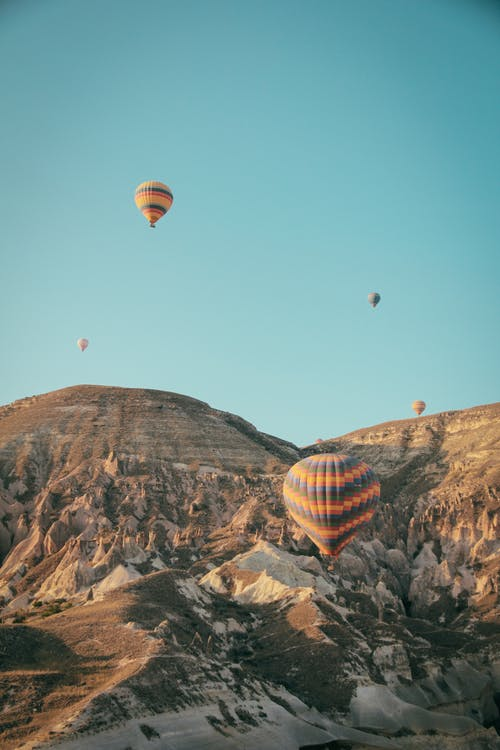
\includegraphics[width=0.5\columnwidth]{Chapters/Chapter1/Figures/Actors_SG}
\caption{Sample Image}
\label{Actors_SG}
\end{figure}


\section{LITERATURE REVIEW} % New Section Format
\subsection{Constituents of Advanced Metering Infrastructure} % New Sub-Section Format
Paragraph text goes here.

\subsubsection*{A. \textit{Advanced Metering Infrastructure}} % New Sub-Sub-Section Format
Advanced metering infrastructure (AMI) is an integrated system of smart energy meters (SEM), communication networks, and meter data management systems (MDMS) that enables bidirectional communication between utilities and consumers [\cite{park2010}]. 

\subsubsection*{B. \textit{Load Monitoring in AMI}}
Paragraph text goes here.

\section{OBJECTIVE AND SCOPE OF THE PRESENT RESEARCH WORK} % Objective and Scope Format
\noindent The objectives of the present research work are as follows:

\begin{enumerate}[itemsep=0.2cm,topsep=1pt,parsep=0pt,partopsep=0pt]
\item First Novel Point
\begin{itemize}[itemsep=0cm,topsep=2pt]
\item supportive statements;
\item benefits;
\end{itemize}
\item Second Novel Point
\begin{itemize}[itemsep=0cm,topsep=2pt]
\item supportive statements;
\item benefits;
\end{itemize}

\end{enumerate}

The scope of the present research work adopts a steady state modeling of household appliances from [\cite{arun2017}]. Replace existing sample paragraphs with your paragraphs.

\section{ORGANIZATION OF THESIS}
\noindent \textbf{Chapter 2:} This chapter deals with.

\noindent \textbf{Chapter 3:} In this chapter. % Path of Chapter 1
\chapter{CHAPTER 2 NAME GOES HERE}
\section{INTRODUCTION}
Paragraph text goes here.

\section{SAMPLE EQUATION ARRAY}
Use align syntax for equation array. Sample has been given below:
\begin{align}
S_{l} &= [s_{l}^{1},s_{l}^{2},...,s_{l}^{t},...,s_{l}^{M}] \quad \forall \ l \in \mathcal{L} 
\label{SLstatus}
\\
s_{l}^{t} &= \left\{ \begin{array}{ll} \begin{array}{ll}
					0 & \mbox{if $l^{th}$ SL is OFF}  \\ 
         			1 & \mbox{if $l^{th}$ SL is ON} \\ \end{array} 
         			& \forall \ l \in \mathcal{L} \\ \end{array} \right. 
\label{SLelem}
\\
\zeta_{l} &\leq \varpi_{l}-\vartheta_{l} \quad \forall \ l \in \mathcal{L}
\label{InputConstraint}
\\
\chi_l &= \left \{ \begin{array}{ll}
			0 & \mbox{for ISL} \\
			1 & \mbox{for NISL} \\
			\end{array} \right.
\label{SLPremption}
\\
P_{SL} &= \sum_{t=1}^{M}{\sum_{l=1}^{N}(s_{l}^{t}.P_{l})}
\label{SLpower}
\end{align}

Similarly, sample table is given below:
\begin{table}[htbp]
\caption{Internal parameters of battery during discharging}
\begin{center}
\renewcommand{\arraystretch}{2} % Alter number to change the width of a row
\setlength\tabcolsep{4pt} % Alter number to change the width of a column
% Help on LaTeX Tables: https://en.wikibooks.org/wiki/LaTeX/Tables
\begin{tabular}{|c|c|c|c|c|c|}
\hline
\textbf{SoC} & \bm{$R_0~(m\Omega)$} & \bm{$R_1~(m\Omega)$} & \bm{$C_1~(kF)$} & \bm{$R_2~(m\Omega)$} & \bm{$C_2~(kF)$} \\
\hline
0	&118.152	&23.49	&0.447601	&2.328	&2.306946\\
10	&116.176	&09.81	&0.377278	&1.417	&1.430313\\ 
20	&116.176	&14.19	&0.340939	&1.982	&1.886134\\
30	&110.702	&10.84	&0.388916	&5.174	&0.772787\\
40	&114.272	&06.23	&0.319658	&3.128	&0.677029\\
50	&112.429	&03.51	&0.838898	&3.371	&0.932269\\
60	&105.512	&05.64	&0.514280	&3.923	&0.753494\\
70	&107.239	&04.64	&0.854056	&1.184	&2.098372\\
80	&105.615	&06.16	&0.503514	&1.885	&2.638010\\
90	&105.512	&06.33	&0.434482	&1.418	&1.766140\\
100	&099.014	&17.08	&0.417306	&4.515	&0.965072\\
\hline
\end{tabular}
\label{T:Discharging}
\end{center}
\end{table} % Path of Chapter 2
% In two side printing, we make sure that the new chapter starts on right side page.
% If previous chapter ends on right side, then one blank side must be added.
% The 3 line command below does the same
\newpage
\thispagestyle{plain} 
\mbox{}
\chapter{CHAPTER NAME GOES HERE}
\section{INTRODUCTION}
DR programs are a portfolio of signaling schemes from the utility to consumers for load shifting/shedding with a given deadline.
   
\section{SAMPLE ALGORITHM} 
Furthermore, the pseudocode depicted in algorithm \ref{C5:A:Priority} explicitly describes the underlying load prioritization subroutine.
% Below given depicts use of algorithm package
% Modify as per the requirement of your algorithm 
% To learn more about modifications, please refer https://en.wikibooks.org/wiki/LaTeX/Algorithms
\begin{algorithm}[!htb]
\caption{Load Prioritization Subroutine}
\label{C5:A:Priority}
\begin{algorithmic}
\State $P_R^t = MDL - P^t$\Comment{\textbf{\textit{Remaining power}}}
\State $j = 1$ \Comment{\textbf{\textit{iterator}}}
\State $X = [i_1,i_2,i_3,........,i_N]$ \Comment{\textbf{\textit{load numbers}}}
\State $Y = [h_1^t,h_2^t,h_3^t,........,h_N^t]$\Comment{{\textbf{\textit{load priority array}}}}
\State $Z = [\{X(1):Y(1)\},\{X(2):Y(2)\},.........,\{X(N):Y(N)\}]$ \Comment{\textbf{\textit{{\{key:value\} pair}}}}
\State $z = [sorted(Z\{key:value\})]$\Comment{\textbf{\textit{descending order of value}}}
\For{$j$ \textit{in range}\ $1$ $\rightarrow$ $length(z)$}
\If {$P_{z[j]}$ $>$ $P_R$}
\State $H[z\{j\}]\gets 0$
\Else
\State $H[z\{j\}]\gets 1$
\EndIf
\State \textbf{end}
\State $P_R^t \gets P_R^t-P_{z[j]}$
\EndFor
\State \textbf{end}
\For{$k$ \textit{in range}\ $1$ $\rightarrow$ $length(H)$}
\If {$H(k)==1$}
\State \texttt{load status} $=$ \texttt{ON}
\Else
\State \texttt{load status} $=$ \texttt{OFF}
\EndIf
\State \textbf{end}
\EndFor
\State \textbf{end}
\end{algorithmic}
\end{algorithm} % Path of Chapter 3
%-------------------------------------------------------------------------------------------
% References in NITT Format.
% This modification should be the last work in the preparation of thesis

\newpage
\chaptermark{REFERENCES}
\centerline{\normalsize\textbf{REFERENCES}}%\\	
\addcontentsline{toc}{chapter}{REFERENCES}
\vspace{-0.5cm}
\begingroup
\let\clearpage\relax
\renewcommand\bibname{}
\setstretch{0.9}
\setlength{\bibsep}{10pt}
\bibliographystyle{NITT} %NITT.bst contains the formatting guidelines
\bibliography{References}
\endgroup
\newpage  % Path of References page
%-------------------------------------------------------------------------------------------
\setboolean{@twoside}{false}	
\phantomsection
\chaptermark{LIST OF PAPERS BASED ON THE THESIS}
\newpage
\centerline{\normalsize\textbf{LIST OF PAPERS BASED ON THE THESIS}}%\\
\addcontentsline{toc}{chapter}{LIST OF PAPERS BASED ON THE THESIS}
\vspace{0cm}
\smallskip
\subsubsection*{Patent Filed}
\begin{enumerate}
\item \textbf{Singh, S.}, \textbf{A. Roy} and \textbf{M.~P. Selvan} Smart Load Node System for Operating an Appliance and Method Thereof. \textit{Intellectual Property India Journal}, March 01, 2019, App No. 201741039083 dated November 2, 2017.    
\end{enumerate}
\subsubsection*{Refereed Journals}
\begin{enumerate}
\item \textbf{Singh, S.}, \textbf{A. Roy} and \textbf{M.~P. Selvan} (2019) Smart load node for nonsmart load under smart grid paradigm: a new home energy management system. \textit{IEEE Consumer Electronics Magazine}, \textbf{8}(2), 22--27.
\end{enumerate}
\subsubsection*{International Conferences}
\begin{enumerate}
\item \textbf{Singh, S.}, \textbf{A. Namboodiri} and \textbf{M.~P. Selvan} (2019) Simplified algorithm for dynamic demand response in smart homes under smart grid environment. \textit{IEEE PES GTD Grand International Conference \& Exposition Asia}, Bangkok, Thailand.
\item \textbf{Singh, S.} and  \textbf{M.~P. Selvan} (2019) A smart energy meter enabling self-–demand response of consumers in smart cities of Tamil Nadu. \textit{International Conference on Smart Cities Model (ICSCM 2019)}, IIT Madras, Chennai, India.
\item  \textbf{Dinesh, P.}, \textbf{K.~K.~Teja}, \textbf{S. Singh}, \textbf{M.~P. Selvan} and \textbf{S. Moorthi} (2018) FPGA Based SoC Estimator and Constant Current Charging/Discharging Controller for Lead--Acid Battery. \textit{IEEE India Council Conference (INDICON)}, Coimbatore, India.
\item \textbf{Singh, S.}, \textbf{Arun S.~L.} and \textbf{M.~P. Selvan} (2017) Regression based approach for measurement of current in single--phase smart energy meter. \textit{2017 IEEE Region 10 Symposium (TENSYMP)}, Cochin, India.
\end{enumerate}
\subsubsection*{Papers Under Review}
\begin{enumerate}
\item \textbf{Singh, S.}, \textbf{S. Thirumalai} and \textbf{M.~P. Selvan} Realization of self-demand response through non-intrusive load monitoring algorithm. \textit{IEEE CONECCT 2019}, IIIT Bangalore.
\end{enumerate} % Path of Publications page
\newpage
\phantomsection
\chaptermark{CURRICULUM VITAE}
\addcontentsline{toc}{chapter}{CURRICULUM VITAE}
\centerline{\normalsize\textbf {CURRICULUM VITAE}}
\vspace{0cm}
\smallskip

\noindent {\large {\textbf{\textsc{Shashank Singh}}}}\\
\texttt{DoB: October 01, 1994}\\
\texttt{Awkash Nagar, Chopan, Sonbhadra, Uttar Pradesh, India - 231205}

\noindent\textbf{\textsc{Educational Qualifications}}

\textbf{\textsc{Master of Science (M.S.) By Research}}, \texttt{2016-Present}
\begin{table}[!htbp]
\begin{tabular}{r c l}
\textit{Institution} & : & National Institute of Technology Tiruchirappalli\\
\textit{University} & : & National Institute of Technology  Tiruchirappalli\\
\textit{Specialization} & : & Electrical and Electronics Engineering \\
\textit{Grade}& : & 9/10
\end{tabular}
\end{table}

\textbf{\textsc{Bachelor of Technology (B.Tech.)}}, \texttt{2010-2014}
\begin{table}[!htbp]
\begin{tabular}{r c l}
\textit{Institution} & : & BBD Northern India Institute of Technology, Lucknow\\
\textit{University} & : & Uttar Pradesh Technical University, Lucknow\\
\textit{Specialization} & : & Electrical and Electronics Engineering\\
\textit{Grade} & : & First Division with Honours
\end{tabular}
\end{table}

\noindent \textbf{\textsc{Research Interests}}

Smart Grids, Demand Response, Embedded Systems, and Internet of Things. % Path of CV page
\newpage
\phantomsection
\chaptermark{GENERAL TEST COMMITTEE}
\addcontentsline{toc}{chapter}{GENERAL TEST COMMITTEE}
\centerline{\normalsize\textbf {GENERAL TEST COMMITTEE}}
\vspace{0cm}
\smallskip
\begin{table}[hbtp]
\centering
\renewcommand{\arraystretch}{1.25}
\begin{tabular}{|p{0.15\textwidth} p{0.8\textwidth}} \hline
 & \multicolumn{1}{|c|}{\textbf{Name of the Chairman}} \\
 & \multicolumn{1}{|c|}{Professor}  \\
\multicolumn{1}{|c}{\textbf{Chairman}}  & \multicolumn{1}{|c|}{\textit{Department of Electrical and Electronics Engineering}}   \\
 & \multicolumn{1}{|c|}{\textit{National Institute of Technology Tiruchirappalli}} \\
 & \multicolumn{1}{|c|}{Tamil Nadu, India -- 620015.}\\ \hline \hline
  & \multicolumn{1}{|c|}{\textbf{Name of the Guide}}\\
 & \multicolumn{1}{|c|}{Associate Professor} \\
\multicolumn{1}{|c}{\textbf{Research Guide}} & \multicolumn{1}{|c|}{\textit{Department of Electrical and Electronics Engineering}}\\
 & \multicolumn{1}{|c|}{\textit{\textit{National Institute of Technology Tiruchirappalli}}} \\
 & \multicolumn{1}{|c|}{Tamil Nadu, India -- 620015.} \\ \hline \hline
 & \multicolumn{1}{|c|}{\textbf{Name of Internal Member}}\\
 & \multicolumn{1}{|c|}{Associate Professor} \\
\multicolumn{1}{|c}{\textbf{Internal Member}} & \multicolumn{1}{|c|}{\textit{Department of Electrical and Electronics Engineering}}\\
 & \multicolumn{1}{|c|}{\textit{National Institute of Technology Tiruchirappalli}} \\
 & \multicolumn{1}{|c|}{Tamil Nadu, India -- 620015.} \\ \hline \hline
 & \multicolumn{1}{|c|}{\textbf{Name of External Member}}  \\
 & \multicolumn{1}{|c|}{Associate Professor} \\
\multicolumn{1}{|c}{\textbf{External Member}}  & \multicolumn{1}{|c|}{\textit{Department of Electrical and Electronics Engineering}} \\
 & \multicolumn{1}{|c|}{\textit{Government College of Technology Coimbatore}} \\
 & \multicolumn{1}{|c|}{Tamil Nadu, India -- 641013.} \\ \hline
\end{tabular}
\end{table} % Path of GTC/DC committee page
%-------------------------------------------------------------------------------------------
\end{document}
%-------------------------------------------------------------------------------------------